\thispagestyle{plain}

\begin{center}
    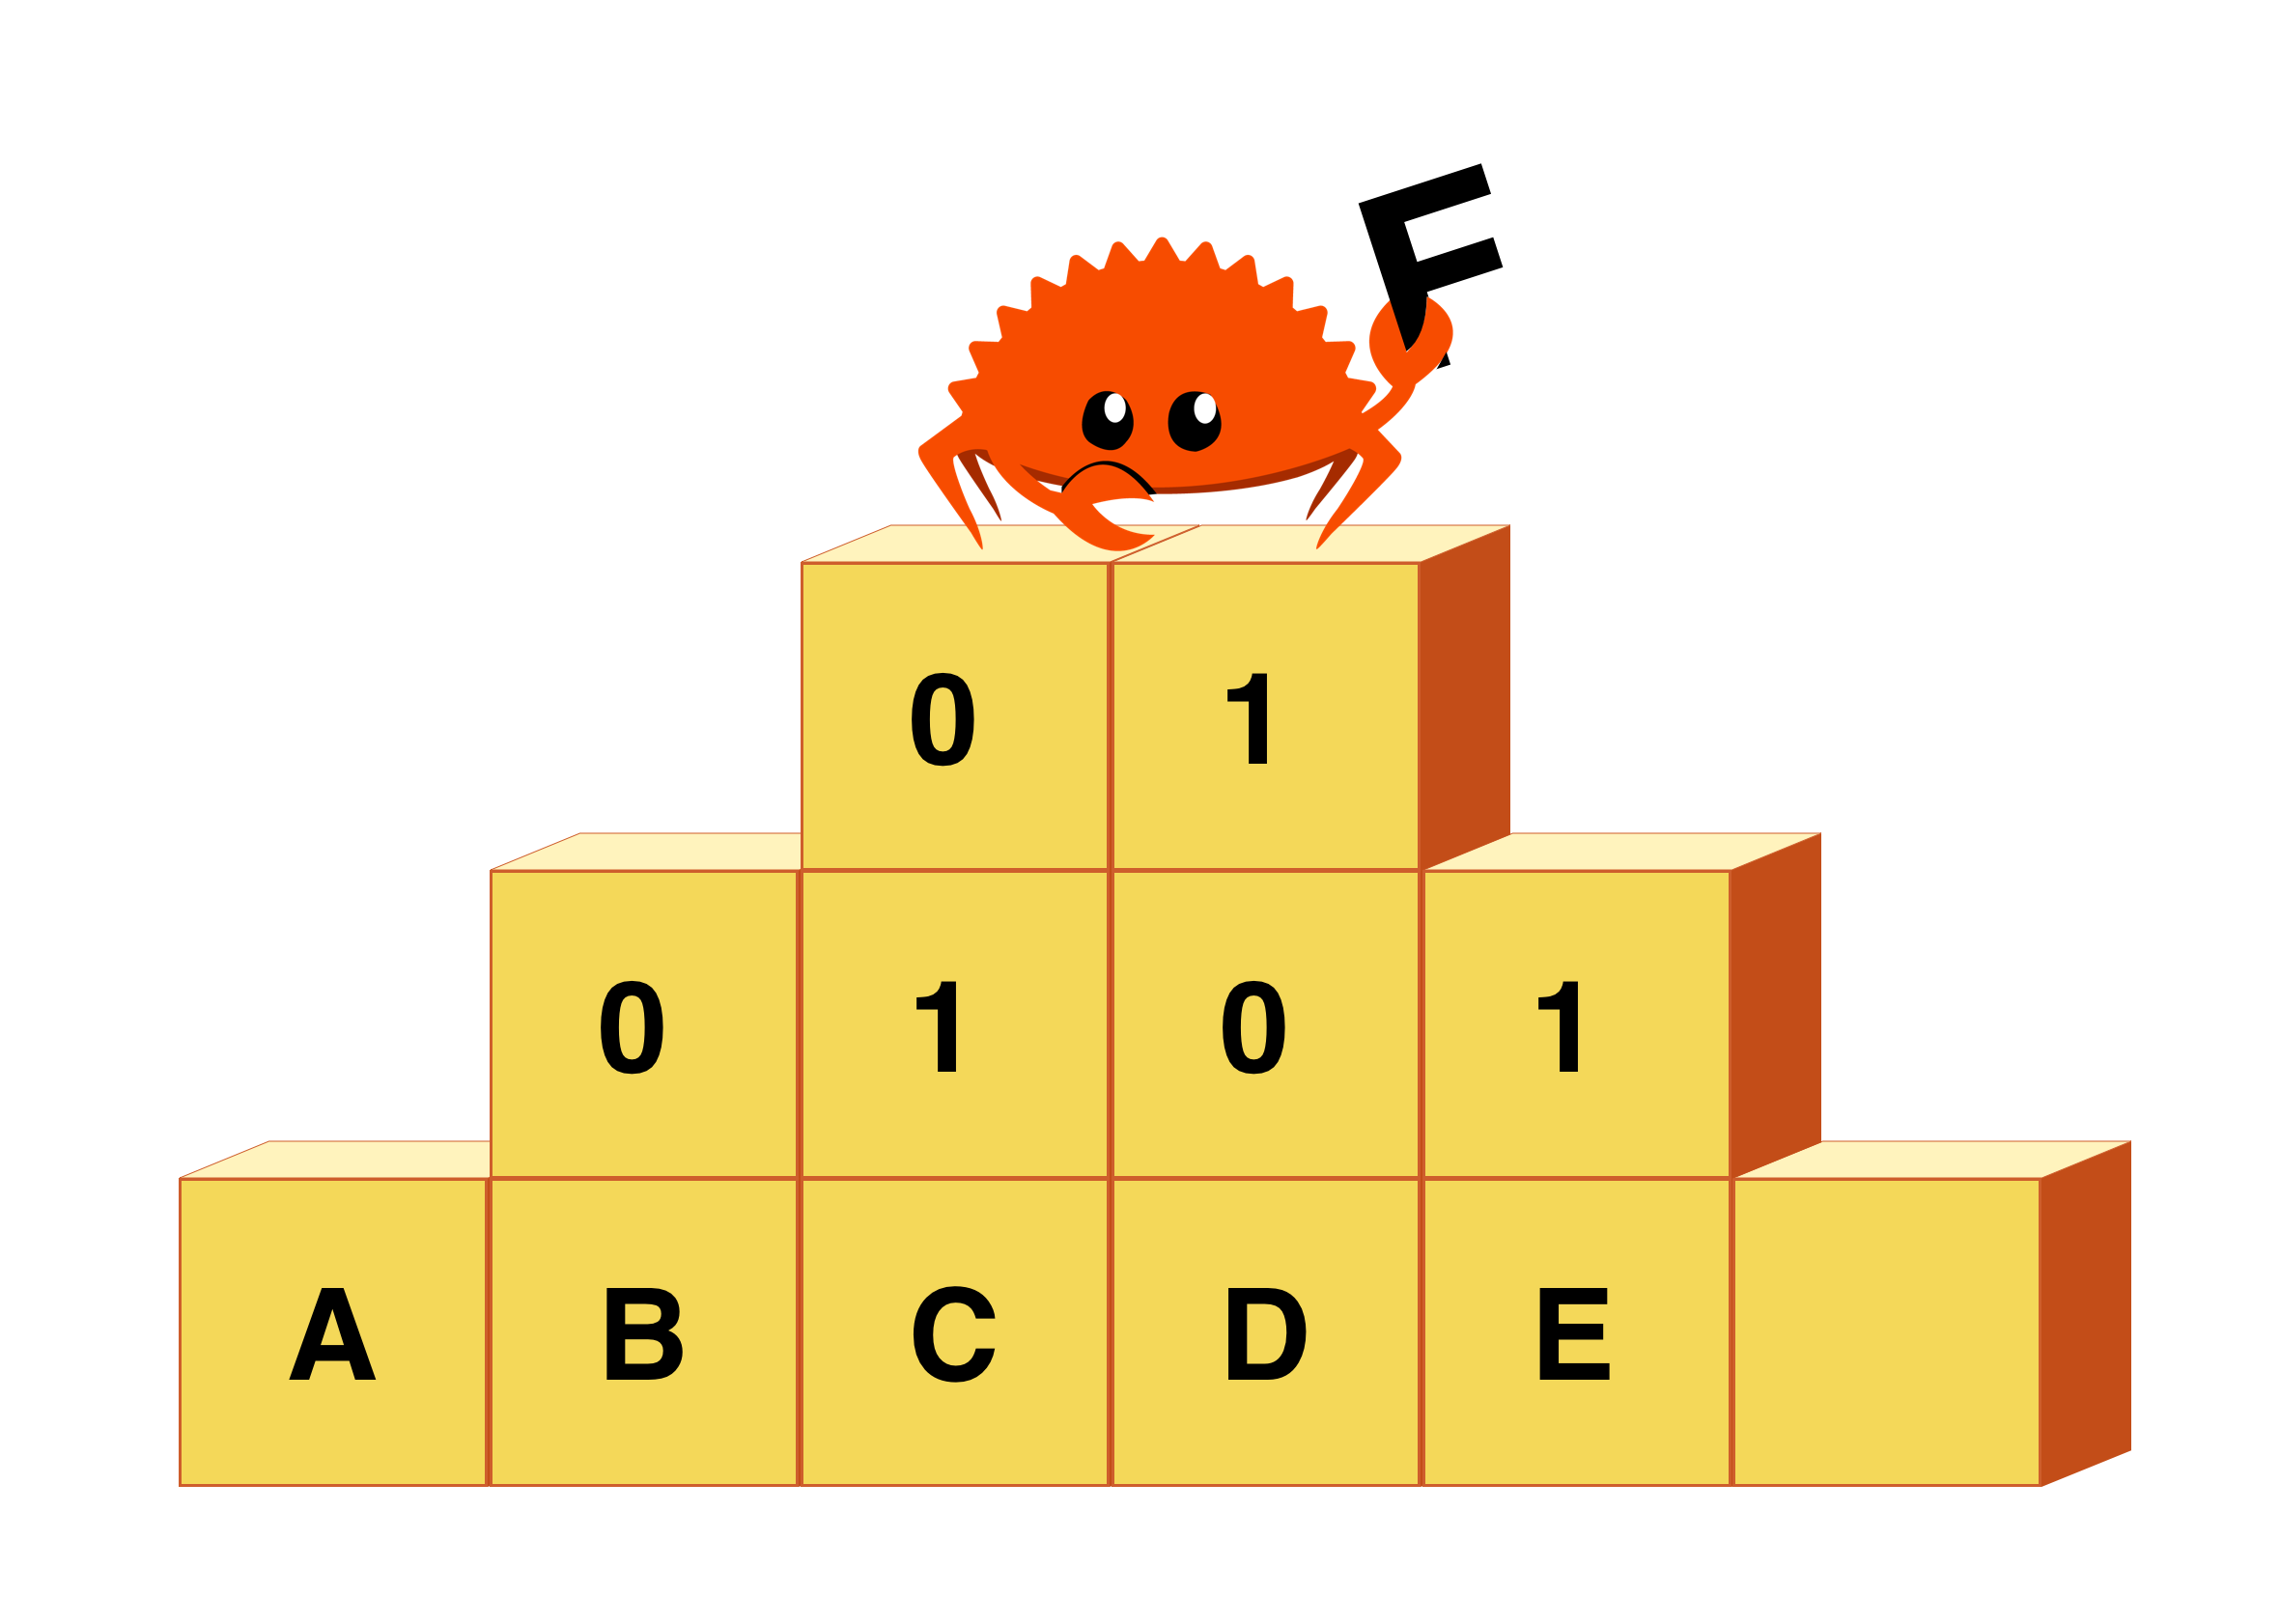
\includegraphics[width=8cm, angle=0, trim=10 10 10 10, clip]{images/ferris-climbing.png}

    \phantomsection
    \addcontentsline{toc}{section}{Reading notes}

    \section*{Reading notes}
    \begin{justify}
        The links to the LaTeX source code and the latest version of this document can be found at \url{https://abishov.com/thesis/}. The implementation, documentation, and visualization demo can be found at \url{https://abishov.com/pvec-rs}.

        If you notice any typos while reading the document, or have any feedback in general, feel free to open an issue at \url{https://github.com/arazabishov/thesis/issues} or send me an email at \href{mailto:araz@abishov.com}{\nolinkurl{araz@abishov.com}}.

        \paragraph{Colophon}
        The illustration above with Ferris\footnote{Unofficial mascot for Rust: \url{https://rustacean.net/}} sitting on top of \treerrb{}, kindly prepared by Vanessa Tesorone. The reading notes design and the idea to use Rust's mascot for the document decoration was inspired by the master's thesis of Erik Vesteraas\footnote{\url{http://erik.vestera.as/thesis/}}.
    \end{justify}

    \subsection*{Typographic conventions}
    \begin{tabular}{ r l }
        Clickable link & \href{https://www.rust-lang.org/}{Rust Programming Language} \\
        Inline code and types & \mintinline{rust}{Vec::new()} \\
        Project or library name & \pvecrs{} \\
    \end{tabular}

\end{center}
